\documentclass[a4paper,12pt]{article}

% Math
\usepackage{amsmath}
\usepackage{amsthm}
\usepackage{thmtools}
\usepackage{amssymb}
\usepackage{calc}
\usepackage{bbm}
\usepackage{commath}
% Other packages
\usepackage{geometry}
\geometry{left=1.5cm,right=1.5cm,top=2cm,bottom=2cm} 
\usepackage{graphicx}
\usepackage{enumitem}
\usepackage{listings}
\usepackage{xcolor}

\definecolor{codegreen}{rgb}{0,0.6,0}
\definecolor{codegray}{rgb}{0.5,0.5,0.5}
\definecolor{codepurple}{rgb}{0.58,0,0.82}
\definecolor{backcolour}{rgb}{0.95,0.95,0.92}

\lstdefinestyle{mystyle}{
    backgroundcolor=\color{backcolour},   
    commentstyle=\color{codegreen},
    keywordstyle=\color{magenta},
    numberstyle=\tiny\color{codegray},
    stringstyle=\color{codepurple},
    basicstyle=\ttfamily\footnotesize,
    breakatwhitespace=false,         
    breaklines=true,                 
    captionpos=b,                    
    keepspaces=true,                 
    numbers=left,                    
    numbersep=5pt,                  
    showspaces=false,                
    showstringspaces=false,
    showtabs=false,                  
    tabsize=2
}

\lstset{style=mystyle}

\usepackage{hyperref}
\hypersetup{
    colorlinks=true,
    linkcolor=blue,
    filecolor=magenta,      
    urlcolor=cyan,
}

\urlstyle{same}

\usepackage[
backend=biber,
style=alphabetic,
sorting=ynt
]{biblatex}
\addbibresource{ref.bib}
\usepackage[nottoc]{tocbibind}

\newcommand{\mbb}[1]{\mathbb{#1}}
\newcommand{\mbbm}[1]{\mathbbm{#1}}
\newcommand{\mbf}[1]{\pmb{#1}}
\title{Stochastic Modelling and Random Processes\\ Problem Sheet 2}
\author{Yiming MA}

\begin{document}
    \maketitle

    \tableofcontents

    \section{Notations}
    \begin{itemize}
        \item All row vectors are represented in a bold font, such as $\mbf{\pi}$, and somtimes, it is also written as $\langle \mbf{\pi} |$ according to the \href{https://en.wikipedia.org/wiki/Bra%E2%80%93ket_notation}{bra–ket notation}.
        
        \item All column vectors are represented with an arrow above, such as $\vec{0}$ which is the vector whose elements are all $0$.
        
        \item Uppercase letters usually represent a matrix, such as $G$.
        
        \item A particular notation, $\mbf{\pi}_t(i)$, means the $i$-th component of the row vector $\mbf{\pi}_t$.
        
        \item $\Delta \in \mathbb{R}^n$ is the region $\{\mbf{x} \in \mathbb{R}^n | \mbf{x} \cdot \vec{1} = 1, \, \mbf{x}_i \ge 0,\, i = 1,\cdots,n\}$.
        
        \item $\mbf{e}_i$ is the row vector whose $i$-th element is $1$, and all other elements are $0$. For example, 
        $$\mbf{e}_1 = [1, 0, \cdots , 0].$$
        (The dimension depends on the context.)
    \end{itemize}

\section{Kingman's Coalescent}
Consider a system of $L$ well mixed, coalescing particles. Each of the $\tbinom{L}{2}$ pairs of particles coalesces independently with rate $1$. This can be interpreted as generating an ancestral tree of $L$ individuals in a population model, tracing back to a single common ancestor.
\begin{enumerate}
    \item[(a)] Let $N_t$ be the number of particles at time $t$ with $N_0 = L$. Give the transition rates of the process $(N_t : t \ge 0)$ on the state space $\{1,\cdots,L\}$. Write down the generator $(\mathcal{L}f)(n)$ for $n \in \{1, \cdots,L\}$ and the master equation. Is the process ergodic? Does it have absorbing states? Give all stationary distributions. 
     
    \textit{ Sol. }  It's easy to see $G_{i,i-1} = \tbinom{i}{2} \times 1 = \tbinom{i}{2}$, for $i \in \{2, \cdots, L\}$. Since $\sum_{j=1}^L G_{i,j} = 0$ and $G_{i,j} = 0$ for $j \notin \{i-1, i\}$, we know $G_{i,i} = - \tbinom{i}{2}$. To summarize,
    \begin{equation}\label{eqn1}
    G_{i,j} = \begin{cases}
        \binom{i}{2} \qquad & j = i - 1, \, i \in \{2, \cdots, L\} \\ 
        -\binom{i}{2} \qquad & j = i, \, i \in \{2, \cdots, L\} \\ 
        0 \qquad & \text{Otherwise}
    \end{cases}.
    \end{equation}
    By $\mathcal{L}(f)(n) = \sum_{k \neq n} G_{n, k} [f(k) - f(n)]$ and \eqref{eqn1}, we know 
    \begin{equation}
        \mathcal{L}(f)(n) = \begin{cases}
            0 \qquad & n = 1 \\ 
            \binom{n}{2}[f(n-1) -f(n)] \qquad & n \in \{2,\cdots, L\}
        \end{cases}.
    \end{equation}
    The master equation is $\frac{\dif}{\dif t} \mbf{\pi}_t(x) = \sum_{y \neq x}\mbf{\pi}_t(y) G_{y,x} - \sum_{y \neq x} \mbf{\pi}_t (x) G_{x,y}$. Use \eqref{eqn1} again, and we get
    \begin{equation}
        \left\{ 
        \begin{array}{l}
            \frac{\dif \mbf{\pi}_t(1)}{\dif t} = \mbf{\pi}_t(2) \\ 
              \\ 
            \frac{\dif \mbf{\pi}_t(i)}{\dif t} = \binom{i+1}{2} \mbf{\pi}_t(i+1) - \binom{i}{2} \mbf{\pi}_t(i),\, i = 2,\cdots,L-1\\ 
             \\ 
            \frac{\dif \mbf{\pi}_t(L)}{\dif t} = -\binom{L}{2} \mbf{\pi}_L
        \end{array}
        \right. 
        .
    \end{equation}

    Obviously, state $1$ is absorbing, and furthermore, it forms an absorbing component $\{1\}$. Thus, the process is SP-ergodic.

    To find all stationary distributions, we need to solve $\mbf{\pi} G = \vec{0}$ with $\mbf{\pi}_t \in \Delta$, which is equivalent to 
    \begin{equation}\label{eqn2}
        \left\{ 
        \begin{array}{l}
            0 \mbf{\pi}_t(1) + \binom{2}{2} \mbf{\pi}_t(2) = 0\\ 
             \\ 
            - \binom{i}{2} \mbf{\pi}_t(i) + \binom{i+1}{2} \mbf{\pi}_t(i+1) = 0, \, i = 2, \cdots, L-1 \\ 
             \\ 
            - \binom{L}{2} \mbf{\pi}_t(L) = 0
        \end{array}
        \right. 
        .
    \end{equation}
    and 
    \begin{equation}\label{eqn3}
        \sum_{i=1}^L \mbf{\pi}_t(i) = 1.
    \end{equation}
    Using backward substitution performed on \eqref{eqn2} results in $\mbf{\pi}_t(i) = 0$, for $i = 2,\cdots, L$. And using \eqref{eqn3}, we have $\mbf{\pi}_t(1) = 1$. So the only stationary distribution is 
    \begin{equation*}
        \mbf{\pi}_t = [\ 1, \, \underbrace{0, \cdots,\, 0}_{(L-1)'s \,0}\ ].
    \end{equation*}
    \item[(b)] Show that the mean time to absorption is given by $\mbb{E}(T) = 2 \left( 1 - \frac{1}{L} \right)$. 
 
    \textit{ Sol. } Let $W_i$ be the holding time for the process to leave state $i$, i.e. $W_i = \inf \{t \in \mathbb{R}_+ | N_t \neq i,\, N_0 = i \}$, for $i = L, L-1, \cdots, 2$. Notice that
    \begin{equation}\label{eqn4}
        T = \sum_{i=2}^L W_i
    \end{equation}
    since the process can only go from state $i$ to $i-1$ at a time.
    
    From lecture, we know $W_i \sim \text{Exponential}(|G_{i,i}|)$. So 
    \begin{equation}\label{eqn5}
        \mathbb{E}[W_i] = \frac{1}{|G_{i,i}|} = \frac{1}{\binom{i}{2}} = \frac{(i-2)! \times 2!}{i!} = \frac{2}{i(i-1)}.
    \end{equation}
    Thus, using \eqref{eqn4} together with the linearity of expectation and \eqref{eqn5}, we get 
    \begin{align*}
        \mathbb{E}(T) = & \mathbb{E} \left(\sum_{i = 2}^L W_i \right) \\ 
        = & \sum_{i = 2}^L  \mathbb{E}(W_i) \\ 
        = & \sum_{i = 2}^L \left( \frac{2}{i(i-1)} \right) \\ 
        = & \sum_{i = 2}^L 2 \left( \frac{1}{i-1} - \frac{1}{i} \right) \\ 
        = & 2 \left(1 - \frac{1}{L} \right).
    \end{align*}

    \item[(c)] Write the generator of the rescaled process $(N_t/L: t \ge 0)$ and Taylor expand it up to the second order. Show that the slowed-down, rescaled process $(X^L_t: t\ge 0)$ where 
    $$X^L_t := \frac{1}{L}N_{\frac{t}{L}},$$
    converges to the process $(X_t: t \ge 0)$ with generator 
    $$\bar{\mathcal{L}}f(x) = - \frac{x^2}{2} f'(x)$$
    and state space $(0, 1]$ with $X_0 = 1$.
    
    Convince yourself that this process is ``deterministic'', i.e. $X_t = \mathbb{E}(X_t)$ for all $t \ge 0$, and compute $X_t$ explicitly. How is your result compatible with the result from (b)?

    \textit{ Sol. } For the rescaled process $(N_t / L: t \ge 0)$, the rates of transitions are not changed, but the state space is replaced with $\{\frac{1}{L}, \cdots, \frac{L}{L}\}$. Thus, the rate matrix is 
    \begin{equation}\label{eqn6}
        G_{i,j} = \begin{cases}
            \binom{iL}{2} \qquad & j = i - \frac{1}{L}, \, i \in \{\frac{2}{L}, \cdots, \frac{L}{L}\} \\ 
            -\binom{iL}{2} \qquad & j = i, \, i \in \{\frac{2}{L}, \cdots, \frac{L}{L}\} \\ 
            0 \qquad & \text{Otherwise}
        \end{cases}
    \end{equation}
    By $(\mathcal{L}f)(n) = \sum_{k \neq n} G_{n,k} [f(k) - f(n)]$ and \eqref{eqn6}, we have 
    \begin{equation}\label{eqn7}
        \mathcal{L}(f)(n) = 
        \begin{cases}
            0 \qquad & n = \frac{1}{L} \\ 
            \binom{nL}{2} [f(n-\frac{1}{L}) - f(n)] \qquad & n \in \{\frac{2}{L}, \cdots, \frac{L}{L}\}
        \end{cases}.
    \end{equation}
    Now Taylor expand \eqref{eqn7} to the sencond order, which results in 
    \begin{equation*}
        \mathcal{L}(f)(n) = 
        \begin{cases}
            0 \qquad & n = \frac{1}{L} \\ 
            \binom{nL}{2} [-\frac{1}{L} f'(n) + \frac{1}{2L^2}f''(n) + o(\frac{1}{L^2})] \qquad & n \in \{\frac{2}{L}, \cdots, \frac{L}{L}\}
        \end{cases}.
    \end{equation*}

    We need to derive the generator of the process $(X_t^L: t \ge 0)$ first. The rate matrix of $(X_t^L: t\ge 0 )$ is 
    \begin{equation}\label{eqn8}
        G_{i,j} = \begin{cases}
            \frac{1}{L}\binom{iL}{2} \qquad & j = i - \frac{1}{L}, \, i \in \{\frac{2}{L}, \cdots, \frac{L}{L}\} \\ 
            -\frac{1}{L}\binom{iL}{2} \qquad & j = i, \, i \in \{\frac{2}{L}, \cdots, \frac{L}{L}\} \\ 
            0 \qquad & \text{Otherwise}
        \end{cases}.
    \end{equation}

    By $(\mathcal{L}f)(n) = \sum_{k \neq n} G_{n,k} [f(k) - f(n)]$ and \eqref{eqn8}, we have 
    \begin{equation}\label{eqn9}
        \mathcal{L}(f)(n) = 
        \begin{cases}
            0 \qquad & n = \frac{1}{L} \\ 
            \frac{1}{L}\binom{nL}{2} [f(n-\frac{1}{L}) - f(n)] \qquad & n \in \{\frac{2}{L}, \cdots, \frac{L}{L}\}
        \end{cases}.
    \end{equation}

    Notice that 
    \begin{eqnarray*}
        \lefteqn{\frac{1}{L} \binom{nL}{2} \left[ f(n - \frac{1}{L}) - f(n)\right]} \\ 
        &=& \frac{1}{L} \cdot \frac{(nL)!}{(nL-2)!2!} \cdot \left[ f(n) - \frac{1}{L} f'(n) + \frac{1}{2L^2} f''(n) + o(\frac{1}{L^2}) - f(n) \right] \\ 
        &=& \frac{1}{L} \cdot \frac{(nL)(nL-1)}{2} \cdot \left[ -\frac{1}{L} f'(n) + \frac{1}{2L^2} f''(n) + o(\frac{1}{L^2}) \right] \\ 
        &=& \frac{n(nL-1)}{2} \cdot \left[ -\frac{1}{L} f'(n) + \frac{1}{2L^2} f''(n) + o(\frac{1}{L^2})\right] \\ 
        &=& \frac{n}{2}\left[ -\frac{nL-1}{L}f'(n) + \frac{nL-1}{2L^2}f''(n) + o(\frac{nL-1}{L^2})\right],
    \end{eqnarray*}
    so as $L \to \infty$, we have 
    $$\lim_{L \to \infty} \frac{1}{L} \binom{nL}{2} \left[ f(n - \frac{1}{L}) - f(n) \right] = - \frac{n^2}{2} f'(n).$$
    In conclusion, we have, as $L \to \infty$, the process $(X_t^L: t \ge 0)$ converges to $(X_t: t \ge 0)$ with generator 
    \begin{equation} \label{eqn10}
        \bar{\mathcal{L}}(f)(x) = - \frac{x^2}{2} f'(x)
    \end{equation}
    and state space $(0, 1]$ with $X_0 = 1$.
    
    \item[(d)] Generate sample paths of the process $(X_t^L: t \ge 0)$ for $L = 10$, $L = 100$, $L = 1000$ and compare to the solution $X_t$ from (c) in a single plot.
      
    \textit{ Sol. }
    \lstinputlisting[language=Python]{problem1d.py}
    The output image is Figure \ref{fig1}.
    \begin{figure}[h!]
        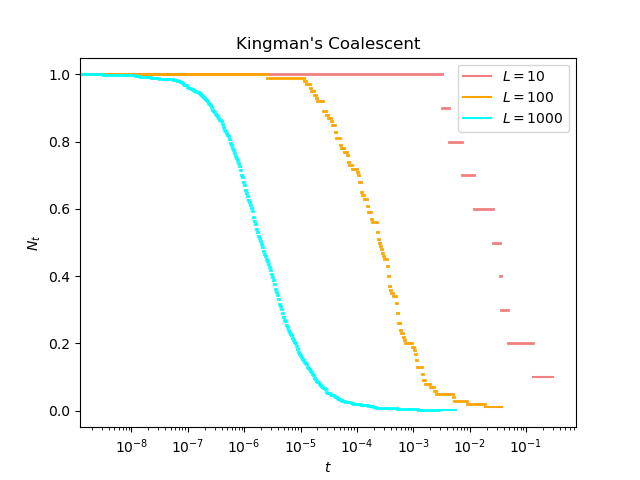
\includegraphics[width=18cm]{Kingman_Coalescent.png}
        \caption{Kingman's Coalescent with $L = 10$, $L = 100$, $L = 1000$}
        \label{fig1}
    \end{figure}
\end{enumerate}
\section{Ornstein-Uhlenbeck Processes}

The Ornstein-Uhlenbeck process $(X_t : t \ge 0)$ is a diffusion process on $\mbb{R}$ with generator 
$$
(\mathcal{L}f)(x) = - \alpha x f'(x) + \frac{1}{2}\sigma^2 f''(x)
$$
with $\alpha,\,\sigma^2 > 0$, and we consider a fixed initial condition $X_0 = x_0$.

\begin{enumerate}
    \item[(a)] Use the evolution equation of expectation values of test functions $f: \mathbb{R} \to \mathbb{R}$
    \begin{equation}\label{eqn11}
        \frac{\dif}{\dif t} \mbb{E} [f(X_t)]  = \mbb{E} [\mathcal{L}f(X_t)],
    \end{equation}
    to derive ODEs for the mean $m(t):=\mbb{E}[X_t]$ and the variance $v(t) := \mbb{E}[X_t^2] - m(t)^2$, and solve them.

    \textit{ Sol. } Set $f(x) = x$ in the evolution equation \eqref{eqn11}, then we have 
    \begin{equation*}
        \frac{\dif}{\dif t} \mbb{E} [X_t]  = \mbb{E} [\mathcal{L}f(X_t)] = \mbb{E} [- \alpha X_t] = -\alpha \mbb{E} [X_t],
    \end{equation*}
    which is 
    \begin{equation}\label{eqn12}
        \frac{\dif m(t)}{\dif t} = - \alpha m(t)
    \end{equation}
    The general solution to \eqref{eqn12} is 
    \begin{equation*}
        m(t) = C \cdot e^{-\alpha t},
    \end{equation*}
    where $C \in \mbb{R}$ is a constant. By $m(0) = \mbb{E}[X_0] = \mbb{E}[x_0] = x_0$, we know $C = x_0$. Thus, the solution to \eqref{eqn12} is 
    \begin{equation}
        m(t) = x_0 \cdot e^{-\alpha t}.
    \end{equation}

    Setting $f(x) = x^2$ in \eqref{eqn11} gives 
    \begin{align}
        \frac{\dif}{\dif t} \mbb{E}[X_t^2] = & \mbb{E} [ - \alpha X_t \cdot 2X_t + \frac{1}{2}\sigma^2 \cdot 2] \notag \\ 
        = & \mbb{E} [ -2 \alpha X_t^2 + \sigma^2] \notag \\ 
        = & -2 \alpha \mbb{E} [X_t^2] + \sigma^2 \label{eqn13}
    \end{align}
    To solve \eqref{eqn13}, we need to find the general solution $h(t)$ of its homogeneous version and a pariticular solution $p(t)$ of it separatively. So $h(t)$ satisfies 
    \begin{equation*}
        \frac{\dif h(t)}{\dif t} = -2 \alpha h(t).
    \end{equation*}
    Using the method of separation of variables again, we know $h(t) = C_1 \cdot e^{-2\alpha t}$, where $C_1 \in \mbb{R}$ is a constant. 

    Now suppose $p(t) = e^{-2\alpha t} + C_2$ with $C_2 \in \mbb{R}$ being a constant. Then we have
    \begin{align*}
        \frac{\dif p(t)}{\dif t} = & -2 \alpha p(t) + \sigma^2 \\ 
        -2 \alpha e^{-2 \alpha t} = & -2 \alpha (e^{-2\alpha t} + C_2 ) + \sigma^2 \\ 
        2 \alpha C_2 = & \sigma^2 \\ 
        C_2 = & \frac{\sigma^2}{2\alpha}.
    \end{align*}
    So a particular solution $p(t)$ is $p(t) = e^{-2\alpha t} +  \frac{\sigma^2}{2\alpha}$.

    Thus, the general solution of \eqref{eqn13} is $\mbb{E} [X_t^2] = C_1 \cdot e^{-2\alpha t} +  \frac{\sigma^2}{2\alpha}$. By $\mbb{E} [X_0^2] = \mbb{E} [x_0^2] = x_0^2$, we have $C_1 = x_0^2 - \frac{\sigma^2}{2\alpha}$. So the second central moment of $X_t$ is 
    $$\mbb{E}[X_t^2] = \left( x_0^2 - \frac{\sigma^2}{2\alpha} \right) e^{-2\alpha t} + \frac{\sigma^2}{2\alpha},$$
    and the variance of $X_t$ is 
    \begin{align*}
        v(t) = & \mbb{E} [X_t^2] - (\mbb{E}[X_t])^2 \\ 
        = &  \left( x_0^2 - \frac{\sigma^2}{2\alpha} \right) e^{-2\alpha t} + \frac{\sigma^2}{2\alpha} - \left( x_0 \cdot e^{-\alpha t} \right)^2 \\ 
        = &  \frac{\sigma^2}{2 \alpha} \cdot \left(1- e^{-2\alpha t} \right).
    \end{align*}

    \item[(b)] Using the fact that $(X_t: t\ge 0)$ is a Gaussian process, give the distribution of $X_t$ for all $t \ge 0$. 
    
    What is the stationary distribution of the process?

    \textit{ Sol. } In (a), we have solved $\mbb{E}[X_t]$ and $\mbb{VAR}[X_t]$:
    $$
    \mbb{E}[X_t] = m(t) = x_0 \cdot e^{-\alpha t} \quad \text{and} \quad \mbb{VAR}[X_t] = v(t) = \frac{\sigma^2}{2 \alpha} \cdot \left(1- e^{-2\alpha t} \right).
    $$
    Since the process $(X_t: t \ge 0)$ is a Gaussian process, we know $X_t$ follows a Gaussian distribution. Thus, 
    $$
    X_t \sim \mathcal{N}\left( x_0 \cdot e^{-\alpha t}, \, \frac{\sigma^2}{2 \alpha} \cdot \left(1- e^{-2\alpha t} \right) \right).
    $$

    From lecture, we know the stationary density of the diffusion process with time-independent $a(y) \in \mbb{R}$ and $\sigma^2(y) > 0$ has the unnormalized stationary density
    $$
    p(x) = \exp\left(\int_0^x \frac{2a(y) - (\sigma^2)'(y)}{\sigma^2(y)} \dif y \right).
    $$
    Since the Ornstein-Uhlenbeck process is a special case of the diffusion process with $a(y) = -\alpha y$ and $\sigma^2(y) = \sigma^2$, we know the unnormalized stationary density of the Ornstein-Uhlenbeck process is 
    \begin{align*}
        p(x) = & \exp\left(\int_0^x \frac{- 2 \alpha y - 0}{\sigma^2} \dif y \right) \\ 
        = & \exp \left(- \frac{\alpha x^2}{\sigma^2} \right) \\ 
        = & \exp \left( - \frac{ (x - 0)^2}{2 \cdot \frac{\sigma^2}{2\alpha} } \right).
    \end{align*}
    So the stationary distribution of the process is $\mathcal{N}(0, \frac{\sigma^2}{2\alpha})$.

    \item[(c)] For $\alpha = 1$, $\sigma^2 = 1$ and $x_0 = 5$, simulate and plot a sample path of the process up to time $t = 10$, by numerically integrating the SDE with time steps $\Delta t = 0.1$ and $\Delta t = 0.01$.
    
    \textit{ Sol. }
    \lstinputlisting[language=Python]{problem2c.py}
    The output image is Figure \ref{fig2}.
    \begin{figure}[h!]
        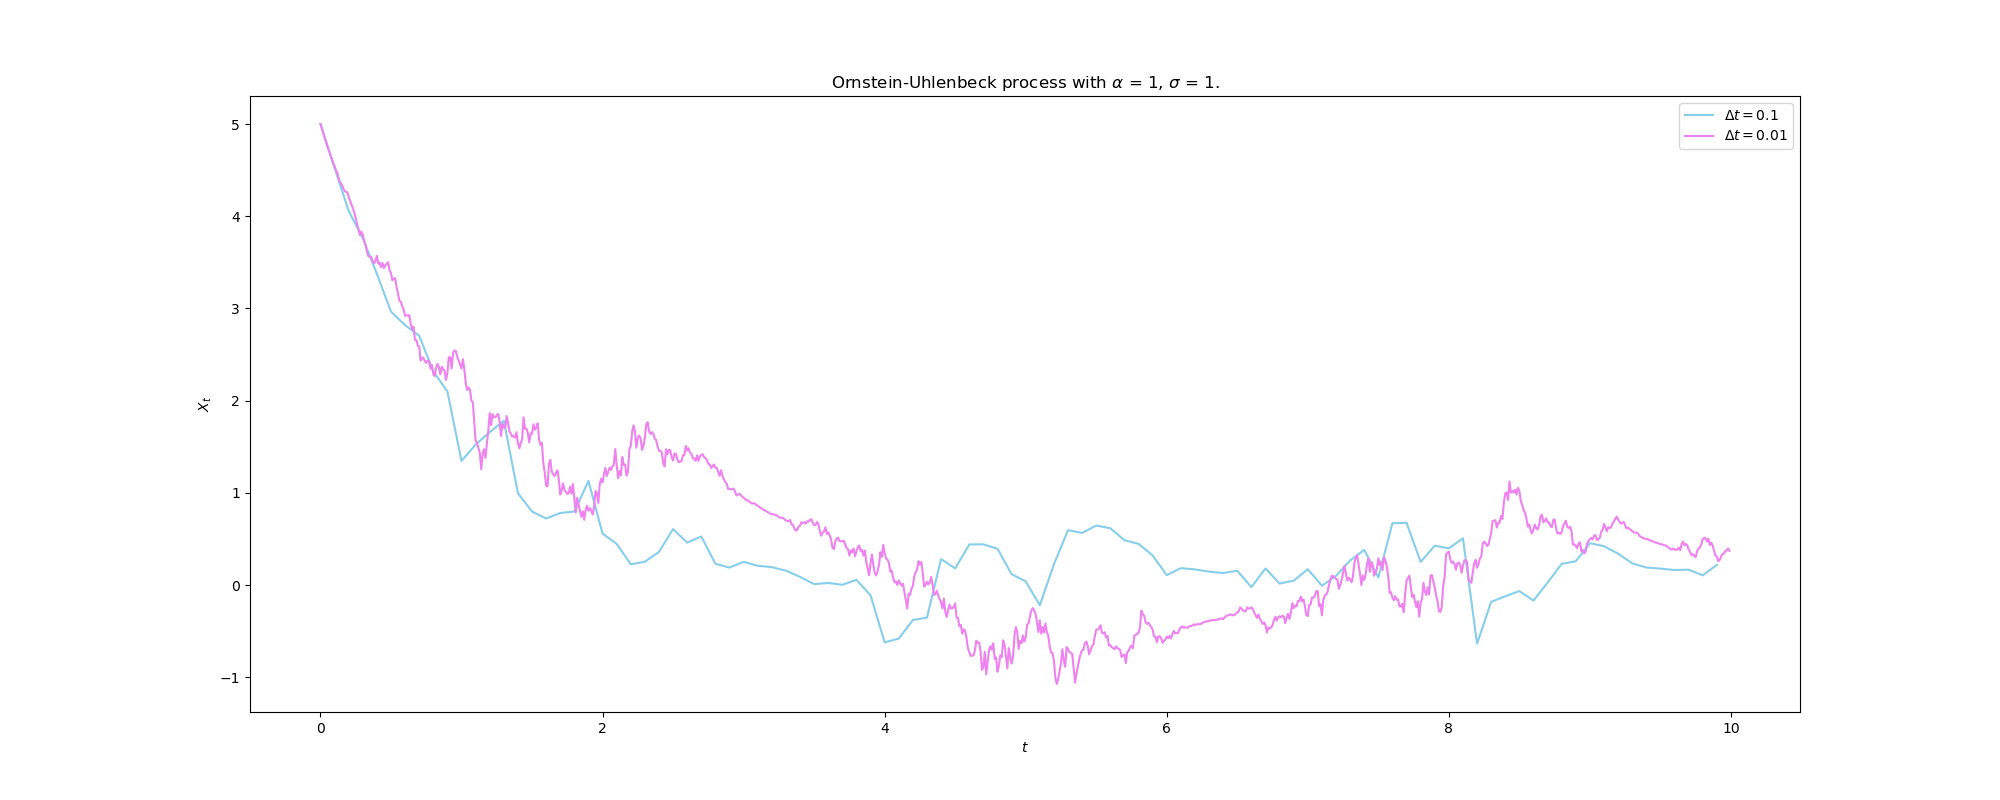
\includegraphics[width=18cm]{Ornstein_Uhlenbeck.png}
        \caption{Ornstein-Uhlenbeck Process with $\alpha = 1$, $\sigma^2 = 1$, $x_0 = 5$}
        \label{fig2}
    \end{figure}
\end{enumerate}

\section{\href{https://en.wikipedia.org/wiki/Moran_process}{Moran Model} and Wright-Fisher Diffusion}

Consider a fixed population of $L$ individuals. At time $t = 0$, each individuum $i$ has a different type $X_0(i)$, and for simplicity, we simply put $X_0(i) = i$. In continuous time, each individuum indepently, with rate $1$, imposes its type on another randomly chosen individuum (or equivalently, kills it and puts its own offspring in its place).

\begin{enumerate}
    \item[(a)] Give the state space of the Markov chain $(X_t: t\ge 0)$. Is it irreducible? What are the stationary distributions?
    
    \textit{ Sol. } Since $X_t(i)$ ($i \in \{1, \cdots, L\}$) is the type of the $i$-th individual at time $t$ and there are $L$ types in total, the state space is $\{1,\cdots,L\}$. 
    
    The process is not irreducible. Suppose at time $t_0$, individual $1$ with type $1$ dies and individual $L$ with type $L$ reproduces to substitute, i.e. 
    $$
    t_0 = \inf \{t > 0: \sum_{i=1}^L \delta_{X_t(i), \, 1} \neq 1\},
    $$
    such that $X_{t_0}(1) = X_{t_0}(L) = L$. Since there are no individuals with tpye $1$ any more, $P_t(1, y) = 0$ for any $t \ge t_0$ and $y \in \{2, \cdots, L\}$.

    Stationary distributions mean once these distributions are entered, the process will stay in them forever. So the stationary distributions of the process are $\mbf{e}_i$, with $i = 1, \cdots, L$.

    \item[(b)] Let $N_t = \sum_{i=1}^L \delta_{X_t(i),\,k}$ be the number of individuals of a given type $k \in \{1, \cdots, L\}$ at time $t$, with $N_0 = 1$.
        \begin{itemize}
            \item Is $(N_t: t \ge 0)$ a Markov process? Given the state space and the generator.

            \textit{ Sol. } The process is obviously Markov, as the distribution of $N_{t_{n+1}}$ given $N_{t_{n}}$, $N_{t_{n-1}}$, $\cdots$, $N_{t_{0}}$ only depends on $N_{t_{n}}$.

            The state space of  $(N_t: t \ge 0)$ is $\{0, 1, \cdots, L\}$.

            Suppose $N_t = i$, where $i \in \{1, \cdots, L-1\}$. Since there are $i$ individuals of type $k$ and each of them reproduces at rate $1$, the total rate of reproduction of individuals of type $k$ is just $i$. Also, we need to select $1$ out of the $L-i$ individuals with other types to be replaced, and this gives the probability $\frac{L-i}{L}$. So 
            $$G_{i,i+1} = \frac{i(L-i)}{L}.$$
            Similarly, we also have 
            $$G_{i,i-1} = \frac{i(L-i)}{L}.$$
            Since $\sum_{j = 1}^{L+1} G_{i,j} = 1$, we know
            $$G_{i,i} = - \frac{2i(L-i)}{L}.$$

            Since state $0$ and state $L$ are absorbing, $G_{0, i} = G_{L, i} = 0$, for any $i \in \{0, \cdots, L\}$.

            Hence, the rate matrix $G$ (indices start from $0$ and end at $L$), whose $(i,j)$ element represents the transition rate from state $i - 1$ into state $j-1$ , is given by 
            $$
            G_{i,j} = \begin{cases}
                \frac{i(L-i)}{L} \qquad & j = i - 1,\, i \in \{1, \cdots, L-1 \} \\ 
                - \frac{2i(L-i)}{L} \qquad & j = i, \, i \in \{1, \cdots, L-1\} \\
                \frac{i(L-i)}{L} \qquad & j = i + 1,\, i \in \{1, \cdots, L-1 \} \\ 
                0 \qquad & \text{Otherwise}
            \end{cases}.
            $$

            \item Is the process irreducible? What are the stationary distributions?
            
            \textit{ Sol. } The process is not irreducible, since state $0$ and state $L$ are absorbing while others are not. Following the same argument in (a), the stationary distributions are $\mbf{e}_0$ and $\mbf{e}_L$.

            \item What is the limiting distribution as $t \to \infty$ for the initial condition $N_0 = 1$?
            
            \textit{ Sol. } As $t \to \infty$, all types have the equal possibility to become the only type of the population. So 
            $$\lim_{t\to\infty}\mbb{P}[N_t = L] = \frac{1}{L}$$
            and 
            $$\lim_{t\to\infty}\mbb{P}[N_t = 0] = \frac{L-1}{L}.$$
        \end{itemize} 
        
        \item[(c)] From now consider general initial conditions $N_0 = n \in \{0, \cdots, L \}$. 
        \begin{itemize}
            \item Compute $m_1(t) = \mbb{E}[N_t]$ for all $t \ge 0$.
            \item Compute $m_2(t) = \mbb{E}[N_t^2]$. What happens in the limit $t \to \infty$?
            \item Compute the absorption probabilities as a function of the initial condition $n$.
        \end{itemize} 

        \textit{ Sol. } To solve $m_1(t)$ and $m_2(t)$, we solve $\mbb{E} [f(N_t)]$ where $f: S := \{0, \cdots, L\} \mapsto \mbb{R}$ first. 
        
        Obviously, the following two statements hold.
        \begin{equation}\label{eqn14}
            \mbb{E}[f(N_t)] = f(0),\quad \text{when } N_0 = 0.
        \end{equation}
        \begin{equation}\label{eqn15}
            \mbb{E} [f(N_t)] = f(L), \quad \text{when } N_0 = L.
        \end{equation}

        Now suppose $N_0 = n \in \{2, \cdots, L-1\}$.
        By $$\mbb{E} [f(N_t)] = \sum_{x \in S} \mbf{\pi}_t(x) f(x) = \langle \mbf{\pi}_t | f \rangle$$ and $$\frac{\dif}{\dif t} \langle \mbf{\pi}_t | = \langle \mbf{\pi}_t | G,$$ 
        we have 
        $$
        \frac{\dif}{\dif t} \mbb{E} [f(N_t)] = \frac{\dif}{\dif t} \langle \mbf{\pi}_t | f \rangle = \langle \mbf{\pi}_t | G | f \rangle = \mbb{E} [ (Gf)(N_t)].$$
        So 
        \begin{align} \label{eqn16}
            \frac{\dif}{\dif t} \mbb{E} [f(N_t)] = & \sum_{k \in S} P_t(n, k) \left( \sum_{j \neq k} G_{k, j}[f(j) - f(k)]\right)  \notag \\ 
            = &  \sum_{k \in S} P_t(n, k) \left(G_{k, k-1} [f(k-1) - f(k)] + G_{k, k+1} [f(k+1) - f(k)] \right) \notag \\ 
            = & \sum_{k \in S} P_t(n, k) \cdot \frac{k(L-k)}{L} \cdot [f(k-1) + f(k+1) - 2f(k)].
        \end{align}
        Set $f(x) = x$ in \eqref{eqn14}, then we have 
        $$
        \frac{\dif}{\dif t} \mbb{E} [N_t] = \sum_{k \in S} P_t(n, k) \cdot \frac{k(L-k)}{L} \cdot [(k-1) + (k+1) - 2k] = 0,
        $$
        which means $m_1(t) = m_1(0) = n$, for $n \in \{2, \cdots, L-1\}$. Along with \eqref{eqn14} and \eqref{eqn15}, we know $m_1(t) = n$, for all $n \in S$.

        Set $f(x) = x^2$ in \eqref{eqn14}, and we get 
        \begin{align}\label{eqn17}
            \frac{\dif}{\dif t}m_2(t)
            = & \frac{\dif}{\dif t} \mbb{E} [N_t^2] \notag \\ 
            = & \sum_{k \in S} P_t(n,k) \cdot \frac{k (L- k)}{L} \cdot [(k-1)^2 + (k+1)^2 -2 k^2] \notag \\ 
            = &  \sum_{k \in S} P_t(n,k) \cdot \frac{k (L- k)}{L} \cdot 2 \notag \\
            = & \frac{2}{L}  \left(L \cdot \sum_{k \in S} P_t(n,k) \cdot k - \sum_{k \in S} P_t(n,k)\cdot k^2\right) \notag \\ 
            = & \frac{2}{L} \cdot \left( L \cdot \mbb{E}[X_t] - \mbb{E}[X_t^2]\right) \notag \\ 
            = & 2 \mbb{E} [X_t] - \frac{2}{L} \mbb{E}[X_t^2]  \notag \\ 
            = & 2n - \frac{2}{L} m_2(t)
        \end{align}
        The general solution to the homogeneous version of \eqref{eqn17} is 
        \begin{equation*}
            h(t) = C_1 e^{-\frac{2}{L}t},
        \end{equation*}
        where $C_1 \in \mbb{R}$ is a constant. Now suppose $p(t) = e^{-\frac{2}{L}t} + C_2$ is a particular solution to \eqref{eqn17}, then 
        \begin{equation*}
            -\frac{2}{L} e^{-\frac{2}{L}t}= \frac{\dif p(t)}{\dif t} = 2n - \frac{2}{L}p(t) = 2n - \frac{2}{L} \left(e^{-\frac{2}{L}t} + C_2 \right),
        \end{equation*}
        which gives $C_2 = nL$. So the general solution to \eqref{eqn17} is 
        \begin{equation*}
            m_2(t) = C_1 e^{-\frac{2}{L}t} + nL.
        \end{equation*}
        By $m_2(0) = \mbb{E} [X_0^2] = \mbb{E}[n^2] = n^2$, we know $C_1 = n^2 - nL = n(n-L)$. Together with \eqref{eqn14} and \eqref{eqn15}, we have 
        \begin{equation}\label{eqn18}
            m_2(t) = n(n-L)e^{-\frac{2}{L}t} + nL.
        \end{equation}
        Let $t \to \infty$ in \eqref{eqn18}, and we have 
        \begin{equation*}
            \lim_{t \to \infty} m_2(t) = nL.
        \end{equation*}

        Let $\tau = \inf\{t \ge 0: N_t \in \{0, L\}\}$, which is the time when the process enters the either one of two absorption states $0$ and $L$. By $\mbb{E} [N_t] = m_2(t) = n$, we have 
        \begin{equation*}
            n = \mbb{E} [N_\tau] = 0 \cdot \mbb{P}[N_\tau = 0] + L \cdot \mbb{P}[N_\tau = L] = L \cdot \mbb{P}[N_\tau = L],
        \end{equation*}
        so $\mbb{P}[N_\tau = L] = \frac{n}{L}$, which is the probability that the process eventually falls in the state $L$. Thus, the probability that the process eventually fixed in the state $0$ is $\frac{L - n}{L}$.
        \item[(d)] Consider the rescaled process $(M_t^L: t \ge 0)$ where 
            $$
            M_t^L = \frac{1}{L} N_{t L^\alpha}
            $$
            on the state space $[0,1]$. For which value of $\alpha > 0$ does $(M_t^L: t \ge 0)$ have a (non-trivial) scaling limit $(M_t: t \ge 0)$?

            Compute the generator of this process and write down the Fokker-Planck equation. (The scaling limit is called \textbf{Wright-Fisher diffusion}.)

        \textit{ Sol. }
        The rate matrix of the rescaled process is 
        $$
            G_{i,j} = \begin{cases}
                i(L-i) L^{\alpha - 1}\qquad & j = i - \frac{1}{L},\, i \in \left\{\frac{1}{L}, \cdots, \frac{L-1}{L} \right\} \\ 
                - 2i(L-i) L^{\alpha - 1} \qquad & j = i, \, i \in \left\{ \frac{1}{L}, \cdots, \frac{L-1}{L} \right\} \\
                i(L-i) L^{\alpha - 1} \qquad & j = i + \frac{1}{L},\, i \in \left\{ \frac{1}{L}, \cdots, \frac{L-1}{L} \right\} \\ 
                0 \qquad & \text{Otherwise}
            \end{cases}.
        $$
        By $(\mathcal{L}f)(X_t) = (Gf)(X_t)$, we have 
        \begin{equation*}
            (\mathcal{L}f)(x) 
            =  \sum_{y \neq x} G_{x,y} [f(y) -f(x)].
        \end{equation*}
        For $x = 0$ and $x = 1$, $(\mathcal{L}f)(0) = (\mathcal{L}f)(1) = 0$. So now suppose $x \in \left\{\frac{1}{L}, \cdots, \frac{L-1}{L}\right\}$, then we have 
        \begin{align}\label{eqn19}
            (\mathcal{L}f)(x) = & x(L-x)L^{\alpha-1} \left[f\left(x+\frac{1}{L}\right) + f\left(x-\frac{1}{L}\right) - 2 f(x) \right] \notag \\ 
            = & x L^\alpha  \left[f\left(x+\frac{1}{L}\right) + f\left(x-\frac{1}{L}\right) - 2 f(x) \right] \notag\\ 
            & - x^2 L^{\alpha-1}  \left[f\left(x+\frac{1}{L}\right) + f\left(x-\frac{1}{L}\right) - 2 f(x) \right]
        \end{align}
        Suppose $f$ is smooth enough to be Taylor expanded into the second order, and perform Taylor expansion of terms involving $f$ in \eqref{eqn19}:
        \begin{align}\label{eqn20}
            f\left(x+\frac{1}{L}\right) + f\left(x-\frac{1}{L}\right) - 2 f(x) = & f(x) + \frac{1}{L}f'(x) + \frac{1}{2L^2} f''(x) + o(\frac{1}{L^2}) \notag \\ 
            & + f(x) - \frac{1}{L}f'(x) + \frac{1}{2L^2} f''(x) + o(\frac{1}{L^2}) \notag \\ 
            & - 2f(x) \notag \\ 
            = & \frac{1}{L^2} f''(x) + o(\frac{1}{L^2})
        \end{align}
        Plug \eqref{eqn20} expansion into \eqref{eqn19}, then we have 
        \begin{equation*}
            (\mathcal{L}f)(x) = x L^{\alpha - 2} f''(x)  - x^2 L^{\alpha - 3}f''(x) + o(L^{\alpha - 2}).
        \end{equation*}
        So in order that the process has a scaling limit, $\alpha > 0$ should satisfy $\alpha -2 \le 0$ and $\alpha - 3 \le 0$ at the same time, which gives $\alpha \in (0, 2]$. $\alpha$ has to be $2$ such that the limiting process is non-trivial, and the corresponding limiting process has the generator 
        \begin{equation*}
            (\bar{\mathcal{L}}f)(x) = x f''(x).
        \end{equation*}

        Now, we are going to derive the Fokker-Planck equation of $(M_t: t \ge 0)$.
        \begin{align}\label{eqn21}
            \frac{\dif}{\dif t} \mbb{E} [f(M_t)] = & \mbb{E} [(\bar{\mathcal{L}}f)(M_t)] \notag \\ 
            \frac{\dif}{\dif t} \int_{0}^1 P_t(x, y) f(y) \dif y = & \mbb{E} [X_t f''(M_t)] \notag \\ 
            \int_0^1 \frac{\partial}{\partial t} P_t(x, y) f(y) \dif y  = &\int_0^1 P_t(x,y) y f''(y) \dif y.
        \end{align}
        Doing integration by parts on the right-hand side of \eqref{eqn21} gives 
        \begin{align}\label{eqn22}
            \int_0^1 P_t(x,y) y f''(y) \dif y = & \int_0^1 P_t(x,y) y \dif f'(y) \notag \\ 
            = & P_t(x,y) y f'(y) |_{y = 0}^{y = 1} - \int_0^1 f'(y) \frac{\partial}{\partial y} (P_t(x,y) y)  \dif y \notag \\ 
            = & P_t(x,y) y f'(y) |_{y = 0}^{y = 1} - \int_0^1 f'(y)  \left( \frac{\partial P_t(x,y)}{\partial y} y + P_t(x,y) \right) \dif y
        \end{align}
        Assuming $ \lim_{t\to\infty} P_t(x,y) = 0$ and $t$ is large enough,  the right-hand side of \eqref{eqn22} becomes 
        \begin{eqnarray}\label{eqn23}
            \lefteqn{P_t(x,y) y f'(y) |_{y = 0}^{y = 1} - \int_0^1 f'(y)  \left( \frac{\partial P_t(x,y)}{\partial y} y + P_t(x,y) \right) \dif y} & & \notag \\ 
            & \approx &  - \int_0^1 f'(y)  \left( \frac{\partial P_t(x,y)}{\partial y} y + P_t(x,y) \right) \dif y \notag \\ 
            & = & - \int_0^1 \frac{\partial P_t(x,y)}{\partial y} y f'(y) \dif y - \int_0^1 P_t(x,y) f'(y) \dif y \notag \\ 
            & = & - \int_0^1 \frac{\partial P_t(x,y)}{\partial y} y \dif f(y) - \int_0^1 P_t(x,y) \dif f(y) \notag \\ 
            & = & - \left. \frac{\partial P_t(x,y)}{\partial y} y f(y) \right\vert_{y=0}^{y=1} + \int_0^1 f(y) \left( \frac{\partial^2 P_t(x,y)}{\partial y^2} y - \frac{\partial P_t(x,y)}{\partial y}\right) \dif y \notag \\ 
            & & - P_t(x,y)f(y) |_{y = 0}^{y = 1} + \int_0^1 \frac{\partial P_t(x,y)}{\partial y} f(y) \dif y \notag \\ 
            & \approx & - \left. \frac{\partial P_t(x,y)}{\partial y} y f(y) \right\vert_{y=0}^{y=1} + \int_0^1 f(y) \left( \frac{\partial^2 P_t(x,y)}{\partial y^2} y - \frac{\partial P_t(x,y)}{\partial y}\right) \dif y \notag \\ 
            & & + \int_0^1 \frac{\partial P_t(x,y)}{\partial y} f(y) \dif y \notag \\ 
            & = & - \left. \frac{\partial P_t(x,y)}{\partial y} y f(y) \right\vert_{y=0}^{y=1} + \int_0^1 f(y) \cdot \frac{\partial^2 P_t(x,y)}{\partial y^2} y \dif y
        \end{eqnarray}
        Also, assume $\lim_{t\to\infty} \frac{\partial P_t(x,y)}{\partial y} = 0$, then in \eqref{eqn23} we have 
        \begin{equation*}
            P_t(x,y) y f'(y) |_{y = 0}^{y = 1} - \int_0^1 f'(y)  \left( \frac{\partial P_t(x,y)}{\partial y} y + P_t(x,y) \right) \dif y \approx \int_0^1 f(y) \cdot \frac{\partial^2 P_t(x,y)}{\partial y^2} y \dif y
        \end{equation*}
        Combined with the \eqref{eqn21}, we have 
        \begin{equation*}
            \int_0^1 \frac{\partial}{\partial t} P_t(x, y) f(y) \dif y \approx \int_0^1 f(y) \cdot \frac{\partial^2 P_t(x,y)}{\partial y^2} y \dif y.
        \end{equation*}
        So the Fokker-Planck equation is 
        \begin{equation}\label{eqn24}
            \frac{\partial}{\partial t} P_t(x,y) = \frac{\partial^2}{\partial t^2} P_t(x,y).
        \end{equation}

        \item[(e)] For the limit process $(M_t: t \ge 0)$ in (d) compute $m(t) = \mbb{E}[M_t]$ and $v(t) = \mbb{E}[M_t^2] - m(t)^2$. Is it a Gaussian process?
        
        \textit{ Sol. } Recall $\frac{\dif}{\dif t}\mbb{E}[f(X_t)] = \mbb{E}[\bar{\mathcal{L}f}(X_t)] = \mbb{E} [X_t f''(X_t)]$. Let $f(x) = x$, then we have 
        \begin{equation*}
            \frac{\dif}{\dif t} \mbb{E} [X_t] = 0.
        \end{equation*}
        So $m(t) = \mbb{E} [M_t] = \mbb{E} [M_0] = m(0)$. 

        Let $f(x) = x^2$, then we have 
        \begin{equation*}
            \frac{\dif}{\dif t}\mbb{E}[M_t^2] = \mbb{E} [2 M_t] = 2 \mbb{E} [M_t] = 2m(t) = 2m(0).
        \end{equation*}
        So $\mbb{E}[M_t^2] = 2m(0) t + \mbb{E}[M_0^2]$, and as a result, $v(t) = \mbb{E}[M_t^2] - (\mbb{E} [M_t])^2 = 2m(0) t + \mbb{E}[M_0^2] - (\mbb{E} [M_0])^2 = 2m(0) t +  \mbb{VAR} [M_0]$.
\end{enumerate}

\section{Birth-Death Process}


A birth-death process $(X_t: t \ge 0)$ is a continuous-time Markov chain with state space $S = \mbb{N}_0 = \{0, 1, \cdots\}$ and jump rates 
$$
x \xrightarrow{\alpha_x} x + 1 \, \text{for all $x \in S$, } x \xrightarrow{\beta_x} x - 1 \, \text{for all $x \ge 1$.}
$$

According to the article \cite{karlin1957classification} of Samuel Karlin and James McGregor, a sufficient and necessary condition for the states of a birth-death process being recurrent is 
\begin{equation}\label{recurrent}
    \sum_{i=1}^\infty \prod_{n=1}^i \frac{\beta_n}{\alpha_n} = \infty,
\end{equation}
sufficient and necessary conditions for them being null recurrent is 
\begin{equation}\label{null recurrent}
    \sum_{i=1}^\infty \prod_{n=1}^i \frac{\beta_n}{\alpha_n} = \infty \quad \text{and} \quad
    \sum_{i=1}^\infty \prod_{n=1}^i \frac{\alpha_{n-1}}{\beta_n} = \infty,
\end{equation}
and sufficient and necessary conditions for them being ergodic is 
\begin{equation}\label{ergodic}
    \sum_{i=1}^\infty \prod_{n=1}^i \frac{\beta_n}{\alpha_n} = \infty \quad \text{and} \quad
    \sum_{i=1}^\infty \prod_{n=1}^i \frac{\alpha_{n-1}}{\beta_n} < \infty,
\end{equation}

\begin{enumerate}
    \item[(a)] Suppose $\alpha_x = \alpha > 0$ for $x \ge 0$ and $\beta_x = \beta > 0$ for $x > 0$. Consider different cases depending on the choice of $\alpha$ and $\beta$ where necessary:
    \begin{itemize}
        \item Is $(X_t: t \ge 0)$ irreducible? Give all communicating classes in $\mbb{N}_0$ and state whether they are transient or null/positive recurrent.
        
        \textit{ Sol. } Since all states are accessible from each other, with positive rates $\alpha$ and $\beta$, all states in $S$ are communicating states. Thus, the process is irreducible.

        $\forall i \ge 1$, $\prod_{n=1}^i \frac{\beta_n}{\alpha_n} = \prod_{n=1}^i \frac{\beta}{\alpha} = \left( \frac{\beta}{\alpha} \right)^i$, so 
        \begin{equation*}
            \sum_{i=1}^\infty \prod_{n=1}^i \frac{\beta_n}{\alpha_n} = \sum_{i=1}^\infty \left( \frac{\beta}{\alpha} \right)^i.
        \end{equation*}
        According to \eqref{recurrent}, these states are recurrent if and only if 
        \begin{equation*}
            \sum_{i=1}^\infty \left( \frac{\beta}{\alpha} \right)^i = \infty,
        \end{equation*}
        which is equivalent to 
        \begin{equation*}
            \frac{\beta}{\alpha} \ge 1.
        \end{equation*}
        Thus, the states are transient if and only if 
        \begin{equation*}
            0 < \frac{\beta}{\alpha} < 1.
        \end{equation*}
        And similarly, by \eqref{null recurrent}, the states are null recurrent if and only if 
        \begin{equation*}
            \frac{\beta}{\alpha} = 1,
        \end{equation*}
        and they are positive recurrent if and only if 
        \begin{equation*}
            \frac{\beta}{\alpha} > 1.
        \end{equation*}
        \item Give all stationary distributions and state whether they are reversible.
        
        \textit{ Sol. } We can use the $\langle \mbf{\pi} | G = \langle \mbf{0} |$ 
        to solve stationary distributions. Notice that 
        \begin{equation*}
            G = 
            \begin{bmatrix}
                - \alpha & \alpha & 0 & 0 & 0 & \cdots \\ 
                \beta & -(\alpha+\beta) & \alpha & 0 & 0 & \cdots \\ 
                0 & \beta & -(\alpha+\beta) & \alpha & 0 & \cdots \\ 
                0 & 0 & \beta & -(\alpha+\beta) & \alpha & \cdots \\ 
                0 & 0 & 0 & \beta & - (\alpha+\beta) & \cdots \\ 
                \vdots & \vdots & \vdots & \vdots & \vdots &  \ddots \\
            \end{bmatrix},
        \end{equation*}
        so 
        \begin{align}
            -\alpha \mbf{\pi}_0 + \beta \mbf{\pi}_1 & = 0 \label{eqn25}\\ 
            \alpha \mbf{\pi}_0 - (\alpha + \beta) \mbf{\pi}_1 + \beta \mbf{\pi}_2 &= 0 \label{eqn26}\\ 
            \alpha \mbf{\pi}_1 - (\alpha + \beta) \mbf{\pi}_2 + \beta \mbf{\pi}_3 & = 0 \label{eqn27}\\ 
            & \vdots \notag
        \end{align}
        To solve these equations, notice that \eqref{eqn25} gives
        \begin{equation}\label{eqn28}
            \beta \mbf{\pi}_1 = \alpha \mbf{\pi}_0.
        \end{equation}
        Plug \eqref{eqn28} into \eqref{eqn26}, and we get 
        \begin{equation}\label{eqn29}
            \beta \mbf{\pi}_2 = \alpha \mbf{\pi}_1.
        \end{equation}
        And pluging \eqref{eqn29} into \eqref{eqn27} results in 
        \begin{equation}
            \beta \mbf{\pi}_3 = \alpha \mbf{\pi}_2.
        \end{equation}
        So we can keep doing this recursively and get 
        \begin{equation*}
            \beta \mbf{\pi}_{n+1} = \alpha \mbf{\pi}_{n}, \quad \forall n \in \mbb{N}_0,
        \end{equation*}
        or equivalently,
        \begin{equation*}
            \mbf{\pi}_n = \left( \frac{\alpha}{\beta} \right)^n \mbf{\pi}_0.
        \end{equation*}
        If $\frac{\alpha}{\beta} \ge 1$, there is no stationary distribution, because 
        \begin{equation*}
            \sum_{n = 0}^\infty \mbf{\pi}_n = \sum_{n = 0}^\infty \left( \frac{\alpha}{\beta} \right)^n \mbf{\pi}_0 \neq 1.
        \end{equation*}
        If $\frac{\alpha}{\beta} < 1$, then solving $\sum_{n = 0}^\infty \mbf{\pi}_n = 1$ gives 
        \begin{equation*}
            \mbf{\pi}_0 = \frac{\beta - \alpha}{\beta},
        \end{equation*}
        so 
        \begin{equation*}
            \mbf{\pi}_n = \left( \frac{\alpha}{\beta} \right)^n \cdot \frac{\beta - \alpha}{\beta}.
        \end{equation*}
        Since $G_{x,y} \mbf{\pi}_x = G_{y,x} \mbf{\pi}_y$ for all $x,y \in S$, the process is time reversible.

        \item Is the process ergodic?
        
        \textit{ Sol. } To check the ergodicity of the process, we only need to verify \eqref{ergodic}.
        \begin{align*}
            \infty = & \sum_{i=1}^\infty \prod_{n=1}^i \frac{\beta_n}{\alpha_n} \\ 
            = & \sum_{i = 1}^\infty \prod_{n=1}^i \frac{\beta}{\alpha} \\ 
            = & \sum_{i = 1}^\infty \left( \frac{\beta}{\alpha} \right)^i,
        \end{align*}
        which holds only when 
        \begin{equation}\label{eqn30}
            \frac{\beta}{\alpha}  \ge 1.
        \end{equation}
        \begin{align*}
            \infty > & \sum_{i=1}^\infty \prod_{n=1}^i \frac{\alpha_{n-1}}{\beta_n}\\ 
            = & \sum_{i=1}^\infty \prod_{n=1}^i \frac{\alpha}{\beta} \\ 
            = & \sum_{i=1}^\infty \left(\frac{\alpha}{\beta} \right)^i
        \end{align*}
        which can be true only when 
        \begin{equation*}\label{eqn31}
            \frac{\alpha}{\beta} < 1
        \end{equation*}
        Based on \eqref{eqn30} and \eqref{eqn31}, the process is ergodic if and only if 
        \begin{equation*}
            \frac{\beta}{\alpha} > 1.
        \end{equation*}
    \end{itemize}

    \item[(b)] Suppose $\alpha_x = x \alpha$, $\beta_x = x \beta$ for $x \ge 0$ with $\alpha,\beta > 0$ and $X_0 = 1$. Consider different cases depending on the choice of $\alpha$ and $\beta$ where necessary: 
    \begin{itemize}
        \item Is $(X_t: t \ge 0)$ irreducible? Give all communicating classes in $\mbb{N}_0$ and state whether they are transient or null/positive recurrent.
        
        \textit{ Sol. } Notice that $\alpha_0 = 0$ and $\beta_0 = \beta > 0$, so state $0$ is absorbing, and thus positive recurrent. For other states, they are communicating. So state space can be decomposed into $\{0\}$ and $\mbb{N}_+$, which means the process is not irreducible.

        Since
        \begin{align*}
            \sum_{i=1}^\infty \prod_{n=1}^i \frac{\beta_n}{\alpha_n} = & \sum_{i=1}^\infty \prod_{n=1}^i \frac{\beta n}{\alpha n} \\
            = & \sum_{i=1}^\infty \prod_{n=1}^i \frac{\beta}{\alpha} \\ 
            = & \sum_{i=1}^\infty \left( \frac{\beta}{\alpha} \right)^i,
        \end{align*}
        by \eqref{recurrent}, states $1, 2, \cdots$ are transient if and only if $\sum_{i=1}^\infty \prod_{n=1}^i \frac{\beta_n}{\alpha_n} < \infty$, which is equivalent to $\frac{\beta}{\alpha} < 1$. 

        Now suppoes $\frac{\beta}{\alpha} \ge 1$ so that states $1, 2, \cdots$ are  recurrent. 
        Since 
        \begin{equation*}
            \sum_{i=1}^\infty \prod_{n=1}^i \frac{\alpha_{n-1}}{\beta_n} = \sum_{i=1}^\infty \prod_{n=1}^i \frac{\alpha(n-1)}{\beta n} = 0 < \infty,
        \end{equation*}
        by \eqref{null recurrent}, states $1, 2, \cdots$ positive recurrent. 

        \item Give all stationary distributions and state whether they are reversible.
        
        \textit{ Sol. } The transition matrix $G$ is
        \begin{equation*}
            \begin{bmatrix}
                0 & 0 & 0 & 0 & 0 & \cdots \\ 
                \beta & -(\alpha + \beta) & \alpha & 0 & 0 & \cdots \\ 
                0 & 2\beta & - 2(\alpha + \beta) & 2\alpha & 0 & \cdots \\ 
                0 & 0 & 3\beta & -3(\alpha + \beta) & 3\alpha & \cdots \\ 
                0 & 0 & 0 & 4\beta & -4(\alpha + \beta) & \cdots \\ 
                \vdots & \vdots & \vdots & \vdots & \vdots & \ddots  
            \end{bmatrix}
        \end{equation*}
        $\langle \mbf{\pi} | G = \langle \mbf{0} |$ gives 
        \begin{align}
            \beta\mbf{\pi}_1 & = 0 \label{eqn32}\\ 
            -(\alpha + \beta) \mbf{\pi}_1 + 2 \beta \mbf{\pi}_2 & = 0 \label{eqn33}\\ 
            \alpha \mbf{\pi}_1 - 2(\alpha + \beta) \mbf{\pi}_2 + 3 \beta \mbf{\pi}_3 & = 0 \label{eqn34}\\ 
            2\alpha \mbf{\pi}_2 - 3(\alpha + \beta) \mbf{\pi}_3 + 4 \beta \mbf{\pi}_4 & = 0 \label{eqn35}\\ 
            & \vdots \notag
        \end{align}
        Solve \eqref{eqn32} first, and this gives $\mbf{\pi}_1 = 0$. Using ``forward-substitution'' in \eqref{eqn33}, \eqref{eqn34}, \eqref{eqn35}, ... gives $\mbf{\pi}_2 = \mbf{\pi}_3 = \mbf{\pi}_4 = \cdots = 0$. Thus, the only stationary distribution is $\mbf{e}_1$, which is 
        \begin{equation*}
            [1, \, 0, \, 0, \, 0, \, \cdots].
        \end{equation*}
        Once being absorbed into state $0$, the process cannot go back into other states, so the process is not time reversible.

        \item Derive an equation for $\mu_t = \mbb{E}[X_t]$ and solve it for initial condition $\mu_0 = 1$.
        
        \textit{ Sol. } For any function $f: S \mapsto \mbb{R}$, 
        \begin{align*}
            (\mathcal{L}f)(x) = & G | f \rangle (x) \\ 
            = & \sum_{y \neq x} G_{x,y} [f(y) - f(x)] \\ 
            = & x \beta [f(x-1) - f(x)] + x \alpha [f(x+1) - f(x)] \\ 
        \end{align*}
        So 
        \begin{align*}
            \frac{\dif}{\dif t} \mbb{E} [f(X_t)] = & \mbb{E} [(\mathcal{L}f)(X_t)] \\ 
            = & \mbb{E} [X_t\beta [f(X_t - 1) - f(X_t)] + X_t \alpha [f(X_t + 1) - f(X_t)]].
        \end{align*}
        Let $f(x) = x$, then we have 
        \begin{align*}
            \frac{\dif}{\dif t} \mbb{E} [X_t] = & \mbb{E} [X_t \beta ( X_t - 1 - X_t) + X_t \alpha (X_t + 1 - X_t)] \\ 
            = & \mbb{E} [- \beta X_t + \alpha X_t] \\ 
            = & (\alpha - \beta)\mbb{E} [X_t], 
        \end{align*}
        whose general solution is give by 
        \begin{equation}\label{eqn36}
            \mbb{E} [X_t] = C e^{(\alpha - \beta) t}.
        \end{equation}
        By the intial condition $\mbb{E} [X_0] = \mu_0 =1$, we know $C = 1$ in \eqref{eqn36}. So the solution is 
        \begin{equation*}
            \mu_t = e^{(\alpha - \beta) t}.
        \end{equation*}

        \item Set up a recursion for the ``extinction probability'' $h_x = \mbb{P}[\lim\limits_{t\to\infty}X_t = 0 | X_0 = x]$ and give the smallest solution with boundary condition $h_0 = 1$.
        
        \textit{ Sol. }
        Since we consider the limit of $X_t$ as $t \to \infty$, it is reasonable to assume $t$ is large enough so that jumps can happen. Obviously, we have $h_0 = 0$, so now assume $x > 0$. 
        
        Let $J_1 = \inf\{t > 0: X_t \neq X_0 \}$ be the time of the first jump, so 
        \begin{equation*}
            \mbb{P}[X_{J_1} = x + 1 | X_0 = x] = \frac{G_{x,x+1}}{|G_{x,x}|} = \frac{x \alpha}{x (\alpha + \beta)} = \frac{\alpha}{\alpha + \beta},
        \end{equation*}
        and 
        \begin{equation*}
            \mbb{P}[X_{J_1} = x - 1 | X_0 = x] = \frac{G_{x,x-1}}{|G_{x,x}|} = \frac{x \beta}{x (\alpha + \beta)} = \frac{\beta}{\alpha + \beta}.
        \end{equation*}
        Now condition on $X_{J_1}$, we have 
        \begin{align}\label{eqn37}
            h_x = & \mbb{P} [\lim_{t\to\infty} X_t = 0 | X_0 = x] \notag \\ 
            = & \mbb{P} [\lim_{t\to\infty} X_t = 0 | X_0 = x, X_{J_1} = x+1] \cdot \mbb{P}[X_{J_1} = x + 1 | X_0 = x] \notag \\ 
            & + \mbb{P} [\lim_{t\to\infty} X_t = 0 | X_0 = x, X_{J_1} = x-1] \cdot \mbb{P}[X_{J_1} = x - 1 | X_0 = x] \notag \\ 
            = & \mbb{P} [\lim_{t\to\infty} X_t = 0 | X_{J_1} = x+1] \cdot \mbb{P}[X_{J_1} = x + 1 | X_0 = x] \notag \\ 
            & + \mbb{P} [\lim_{t\to\infty} X_t = 0 | X_{J_1} = x-1] \cdot \mbb{P}[X_{J_1} = x - 1 | X_0 = x] \quad \text{(by the Markov property)} \notag \\ 
            = & \mbb{P} [\lim_{t\to\infty} X_t = 0 | X_{0} = x+1] \cdot \mbb{P}[X_{J_1} = x + 1 | X_0 = x] \notag \\ 
            & + \mbb{P} [\lim_{t\to\infty} X_t = 0 | X_{0} = x-1] \cdot \mbb{P}[X_{J_1} = x - 1 | X_0 = x] \quad \text{(by homogeneity)} \notag \\ 
            = & h_{x+1} \cdot \frac{\alpha}{\alpha + \beta}  +  h_{x-1} \cdot \frac{\beta}{\alpha + \beta}
        \end{align}
        The characteristic equation of \eqref{eqn37} is 
        \begin{align*}
            t^2 \cdot \frac{\alpha}{\alpha + \beta} + \frac{\beta}{\alpha + \beta} & = t \\ 
            \alpha t^2 - (\alpha + \beta) t + \beta & = 0 \\ 
            (\alpha t - \beta) (t - 1) & = 0,
        \end{align*}
        whose roots are 
        \begin{equation*}
            t_1 = \frac{\beta}{\alpha} \quad \& \quad t_2 = 1.
        \end{equation*}
        If $\alpha = \beta$, then $t_1 = t_2 = 1$, and the general solution to \eqref{eqn37} is 
        \begin{align*}
            h_n = & a \cdot 1^n + b \cdot n \cdot 1^2 \\ 
            = & a + bn,
        \end{align*}
        where $a,\,b\in\mbb{R}$ are two constants. By $h_0 = 1$, we have $a = 1$, so $h_x = 1 + bx$. But $h_x$ is a probability, which means it should range between $0$ and $1$, so we have $b = 0$. So in the case of $\alpha = \beta$, $h_x \equiv 1$.

        Now suppose $\alpha \neq \beta$, so $t_1 \neq t_2$. Then the general solution to \eqref{eqn37} is 
        \begin{align*}
            h_n = & a \cdot 1^n + b \cdot \left( \frac{\beta}{\alpha} \right)^n \\ 
            = & a + b \left( \frac{\beta}{\alpha} \right)^n,
        \end{align*}
        where $a,\,b\in\mbb{R}$ are two constants. Again, use the boundary condition $h_0 = 1$, and we have $a = 1 - b$. Thus, 
        $$h_x = 1 - b + b \left( \frac{\beta}{\alpha} \right)^x.$$

        If $\beta > \alpha$, then $\frac{\beta}{\alpha} > 1$, and as a result, 
        $\lim_{x \to \infty} (\beta / \alpha)^n = \infty$. In order that $h_x$ is a probability, $b$ has to be $0$. So in this case $h_x \equiv 1$. 

        If $\beta < \alpha$, then $\frac{\beta}{\alpha} < 1$, and thus, $(\beta / \alpha)^x le 1$ for all $x \ge 0$. To ensure $h_x \le 1$, let
        \begin{align*}
             1 - b + b \left( \frac{\beta}{\alpha} \right)^x \le & 1 \\ 
             \left( \left( \frac{\beta}{\alpha} \right)^x - 1 \right) b \le & 0\\
             b \ge & 0.
        \end{align*}
        In order to make $h_x$ nonnegative, we need 
        \begin{align*}
            0 \le & 1 - b + b \left( \frac{\beta}{\alpha} \right)^x \\
            1 \ge & \left(1 - \left( \frac{\beta}{\alpha} \right)^x \right) b \\
            b \le & \frac{1}{1 - \left( \frac{\beta}{\alpha}\right)^x} \\ 
            b \le & 1.
        \end{align*}
        So the range of $b$ is $[0, 1]$.

        To conclude, the solution to \eqref{eqn37} is 
        \begin{equation*}
            h_x = \begin{cases}
                1 \qquad & \beta \ge \alpha > 0\\ 
                1 - b + b \left( \frac{\beta}{\alpha} \right)^x \qquad & 0 < \beta < \alpha
            \end{cases},
        \end{equation*}
        where $b \in [0, 1]$ is a constant.

        Obviously, we have made $1 - b + b \left( \frac{\beta}{\alpha} \right)^x \le 1$ when we determined the range of $b$, so the smaller solution is 
        $$
        1 - b + b \left( \frac{\beta}{\alpha} \right)^x,
        $$
        with $0 < \beta < \alpha$ and $b \in [0, 1]$. Let 
        $H(b) = 1 - b + b \left( \frac{\beta}{\alpha} \right)^x$, then 
        $$H'(b) = -1 + \left( \frac{\beta}{\alpha} \right)^x \le 0,$$
        which means $H(b)$ is monotonically decreasing in $[0, 1]$. So the smallest solution is reached when $b = 1$, and in this circumstance, 
        $$h_x = \left( \frac{\beta}{\alpha} \right)^x.$$

        \item Is the process ergodic?
        
        \textit{ Sol. } 
        By \eqref{ergodic}, the process is ergodic if and only if 
        \begin{equation*}
            \sum_{i=1}^\infty \prod_{n=1}^i \frac{\beta_n}{\alpha_n} = \infty \quad \text{and} \quad
            \sum_{i=1}^\infty \prod_{n=1}^i \frac{\alpha_{n-1}}{\beta_n} < \infty.
        \end{equation*}
        The first condition is 
        \begin{align*}
            \infty & = \sum_{i=1}^\infty \prod_{n=1}^i \frac{\beta_n}{\alpha_n} \\ 
            & = \sum_{i=1}^\infty \prod_{n=1}^i \frac{\beta n}{\alpha n} \\ 
            & = \sum_{i=1}^\infty \prod_{n=1}^i \frac{\beta}{\alpha} \\ 
            & = \sum_{i=1}^\infty \left( \frac{\beta}{\alpha} \right)^i,
        \end{align*}
        which is equivalent to $\beta \ge \alpha$. 

        As for the second condition, we have 
        \begin{equation*}
            \sum_{i=1}^\infty \prod_{n=1}^i \frac{\alpha_{n-1}}{\beta_n} = \sum_{i=1}^\infty \prod_{n=1}^i \frac{\alpha(n-1)}{\beta n} = 0 < \infty.
        \end{equation*}
        
        So the process is ergodic if and only if $\beta \ge \alpha$.
    \end{itemize} 
\end{enumerate}

\printbibliography[type=article,title={Reference}]
\end{document}